\begin{figure*}[h]                                                           
 
\includegraphics[width=\linewidth]{./media/images/world_map}%
  \scriptsize{\textsc{\\removing the burden} to implement every detail goes a
    long way toward creating polished \textsc{if} environments}
  \label{fig:editorial}%                                                 
\end{figure*}                                                                

\begin{quotation} 
  \noindent\color{Sepia}{\textit{\textbf{“If you put yourself in a position where you have to stretch outside your comfort zone, then you are forced to expand your consciousness.”}}}\\[.5mm]
   \hfill\color{Sepia}{\small{\textendash Les Brown}}
\end{quotation} 
\newpage
\lettrine[lines=3]{\color{BrickRed}N}{\enspace atural Language Processing}
[\textsc{nltk}] may hold the key to breakthrough levels of engagement in
\textsc{if}. It's power lies in it's ability to query
millions of lines of text, retrieve quantified answers in the source
material, and bring relationships between entities to light. The context
suggestions translate into actionable intelligence
for the author and greater submersion for the reader. \textsc{nltk}'s
ability to retrieve massive numbers of contexts and relationships in seconds
make it's techniques powerful instruments for building immersive world models.

\marginnote{\href{http://sapir.psych.wisc.edu/programming_for_psychologists/cheat_sheets/Text-Analysis-with-NLTK-Cheatsheet.pdf}{Text analysis with \textsc{nltk} cheatsheet}}[2em]
\textsc{nltk} is not only fast it's architecture lends itself to automation.
Once the author selects the topics to be covered\textemdash likely using topic modeling
as described beginning on page \pageref{sec:topic}\textemdash an article summarizer is
used to pull out each topics' salient features.
These results are fed into \textsc{nltk} for context, parts\textendash
of\textendash speech, and related associations specific to each result. Natural
language processing with \textsc{nltk}'s modular architecture provides volumes of
relevant results that can be molded to suit your workflow.

%TODO: Link to nltk cheatsheet

Responses for all kinds of player queries can be 
built efficiently using \textsc{nltk}'s features:
\begin{itemize}
  \setlength\itemsep{0em}
  \item{Varying, sometimes wide\textendash ranging contexts for a particular topic or object}
  \item{Brings forward parser responses you may not have considered}
  \item{Tags objects mentioned in the main prose to avoid ``I don't see any x
      here'' here messages}
\end{itemize}
%I'll outline examples of each with examples and provide a brief tutorial for
%configuring your system to run \textsc{nltk}.
\section{a time and a place}
\marginnote{Corpos: nothing more than a large body of text, sometimes referred to as, ``a big bag of words''}[1em]
Suppose we're writing a character modeled after Captain Ahab in the seminal
classic, ``Moby Dick.'' After loading the Moby Dick corpus, included with
\textsc{nltk}, we query the system for where Captain Ahab appears in context:
\pagebreak

\marginnote{These results appear as broken English because the corpus is processed to remove ``stop words,'' i.e. ``the, a, that,'' etc. Run your queries against raw corpus text if you want results in complete sentences.}[5em]
\begin{lstlisting}
  >>> text1.concordance('ahab')

, eh ? Have ye clapped eye on Captain Ahab ?" " Who is Captain Ahab , sir ?" " A
e on Captain Ahab ?" " Who is Captain Ahab , sir ?" " Aye , aye , I thought so .
 " Aye , aye , I thought so . Captain Ahab is the Captain of this ship ." " I am
ast backing out . Clap eye on Captain Ahab , young man , and thou wilt find that
ptain Peleg , inquiring where Captain Ahab was to be found . " And what dost tho
 " And what dost thou want of Captain Ahab ? It ' s all right enough ; thou art
l thee . He ' s a queer man , Captain Ahab -- so some think -- but a good one .
 , ungodly , god - like man , Captain Ahab ; doesn ' t speak much ; but , when h
ll listen . Mark ye , be forewarned ; Ahab ' s above the common ; Ahab ' s been
ewarned ; Ahab ' s above the common ; Ahab ' s been in colleges , as well as ' m
\end{lstlisting}

From the results we can see that he is a Captain of a ship, educated, is ``above
the common,'' and keeps his thoughts close to his chest overall. Immediately we
find that we can ask Ahab about topics like his ship, his education, and his mission (if he'll
tell us). If we observe closely, we find clues to his personality. This phrase
is intriguing:
\begin{lstlisting}
  , ungodly , god - like man , Captain Ahab ; doesn ' t speak much ; but , when h
\end{lstlisting}

Let's learn more

\begin{lstlisting}
  >>> text1.concordance('speak')
 ' t speak much ; but , when he does speak , then you may well listen . Mark ye
\end{lstlisting}
According to at least one character in the book (who knows Capatain Ahab well as
other queries attest), Captain Ahab is a quiet man but should be listened to
when he does speak.

Notice through shaping our character so far we've not had to ``think'' of
anything\textemdash the system digs through the corpus and provides us with a profile for
our subject of interest.


\includepdf[scale=1.01]{media/images/sailor_ad.pdf}
\section{saving mimesis}
Alright, so we write our character based on Captain Ahab. Let's call him
``Captain Moby'' (sacrilege, I know):
\begin{quote}
Captain Moby leans slightly forward as he scans the horizon from the fore deck
of his ship, ``\textit{Pequod.}'' 
\end{quote}
  An interaction like this would break nimesis:
  \begin{lstlisting}
    > examine Pequod
    I don't see any Pequod here.
  \end{lstlisting}
\marginnote{\href{http://pdf.textfiles.com/books/iftheorybook.pdf}{Roger Sorolla, ``Crimes Against Mimesis'' {\textsc{(pdf)}}}}[1em]
\textsc{nltk} can help with this by taking our prose through a parts\textendash of\textendash speech parser:

\begin{lstlisting}%[basicstyle=\tiny]
>>> mytext = nltk.word_tokenize("Captain Moby leans slightly forward as he scans the horizon from the fore deck of his ship, Pequod.")
>>> nltk.pos_tag(mytext)
[('Captain', 'NNP'), ('Moby', 'NNP'), ('leans', 'VBZ'), ('slightly', 'RB'), ('forward', 'RB'), ('as', 'IN'), ('he', 'PRP'), ('scans', 'VBZ'), ('the', 'DT'), ('horizon', 'NN'), ('from', 'IN'), ('the', 'DT'), ('fore', 'NN'), ('deck', 'NN'), ('of', 'IN'), ('his', 'PRP\$'), ('ship', 'NN'), (',', ','), ('Pequod', 'NNP'), ('.', '.')]
\end{lstlisting}
Here we're looking for Proper nouns (NNP), and nouns (NN). In seconds we're
provided the following actionable items:
\begin{multicols}{2}
\begin{itemize}\setlength\itemsep{0em}
  \item Captain
  \item Moby
  \item horizon
  \item fore
  \item deck
  \item ship
  \item Pequod
\end{itemize}
\end{multicols}
\marginnote{\href{https://www.smithsonianmag.com/history/the-true-life-horror-that-inspired-moby-dick-17576/}{Fun fact: Moby Dick is based on a true story about Captain George Pollard Jr.}}[1em]
\noindent Does the system respond reasonably to, \emph{``examine Pequod''} or
\emph{``examine fore''}? Using the parts\textendash of\textendash speech tager,
yes, we're able to cover all relevant areas in each passage's prose. Your work's
manuscript can be used as input to produce a list of objects for implementation,
perhaps even, creating object templates that have ``TODO'' placed in them saving you the trouble of having to
write it yourself.

If we run an \textsc{nltk} 'similar' query like we did above on the word,
\emph{pequod}, by the way, we get this:
\pagebreak
\begin{lstlisting}
>>> text1.concordance('pequod',lines=10)
Displaying 10 of 25 matches:
...
rare old craft as this same rare old Pequod . She was a ship of the old school ,
to me and Captain Bildad to see the Pequod fitted out for the voyage , and supp
aling I must , and I would ; and the Pequod was as good a ship as any -- I thoug
...
\end{lstlisting}
We now see that the \emph{Pequod} is a commissioned ship of the stoutest breed
of ``old schol'' nautical design and construction.

Notice that the character in our story is modeled from a single
corpus. You can also craft your character with references from several bodies of
work. Other characters can be modeled after completely
separate works; the antagonist in your story could be modeled after
Shakespeare's \textit{Othello}. There are virtually endless ways of customizing
your source material in your work of \textsc{if}.
\section{installation}
Fortunately, installing \textsc{nltk} is fairly straightforward; you need only
python, \textsc{nltk}, and \textsc{nltk-data} installed to use the examples
described here.

\subsection{installing python}
Linux systems, almost without exception \textit{will} have \textsc{python} and \textsc{nltk}
packages available as standard. Here are the commands to install \textsc{python}
for various distributions:\\[1em]
For Debian/Ubuntu:
\begin{lstlisting}
  sudo apt-get install python3 python3-pip
\end{lstlisting}
For Arch Linux:
\begin{lstlisting}
  sudo pacman -S python python-pip
\end{lstlisting}
\marginnote{\href{https://www.python.org/downloads/windows/}{Python for windows download page}}[0.5em]
Windows systems may download \textsc{python} from the link found in the margin notes on this page. I
recommend using 
\textsc{powershell} when working with \textsc{python} and
\textsc{nltk}.Alternatively, in environments where Windows must be used as the
base operating system, it’s best to run these applications inside a virtual
machine running linux or bsd for industrial grade text processing.
\marginnote{\href{https://docs.python.org/3/using/windows.html}{Python documentation, ``Python on Windows''}}[-2em]
\subsection{installing nltk}
It's almost always better to stay inside the distribution's method for
installing \textsc{python} applications without resorting to \textsc{pip} or
other \textsc{python}
installation systems. Conflicts will occur if a dependency is
installed with \textsc{pip} when the package manager finds that the dependency is already installed. For \textsc{nltk} the installation looks like this:\\[1em]
For Debian/Ubuntu:
\begin{lstlisting}
  sudo apt-get install python-nltk 
\end{lstlisting}
For Arch Linux:
\begin{lstlisting}
  sudo pacman -S python-nltk nltk-data
\end{lstlisting}

For all operating systems I recommend downloading all the available
\textsc{nltk} packages; you will save a lot of time later not having to
worry about whether or not a required package is installed for a given
\textsc{nltk} operation:
\begin{lstlisting}
>>> import nltk
>>> nltk.download()
\end{lstlisting}
\begin{figure*}[ht]
\centering
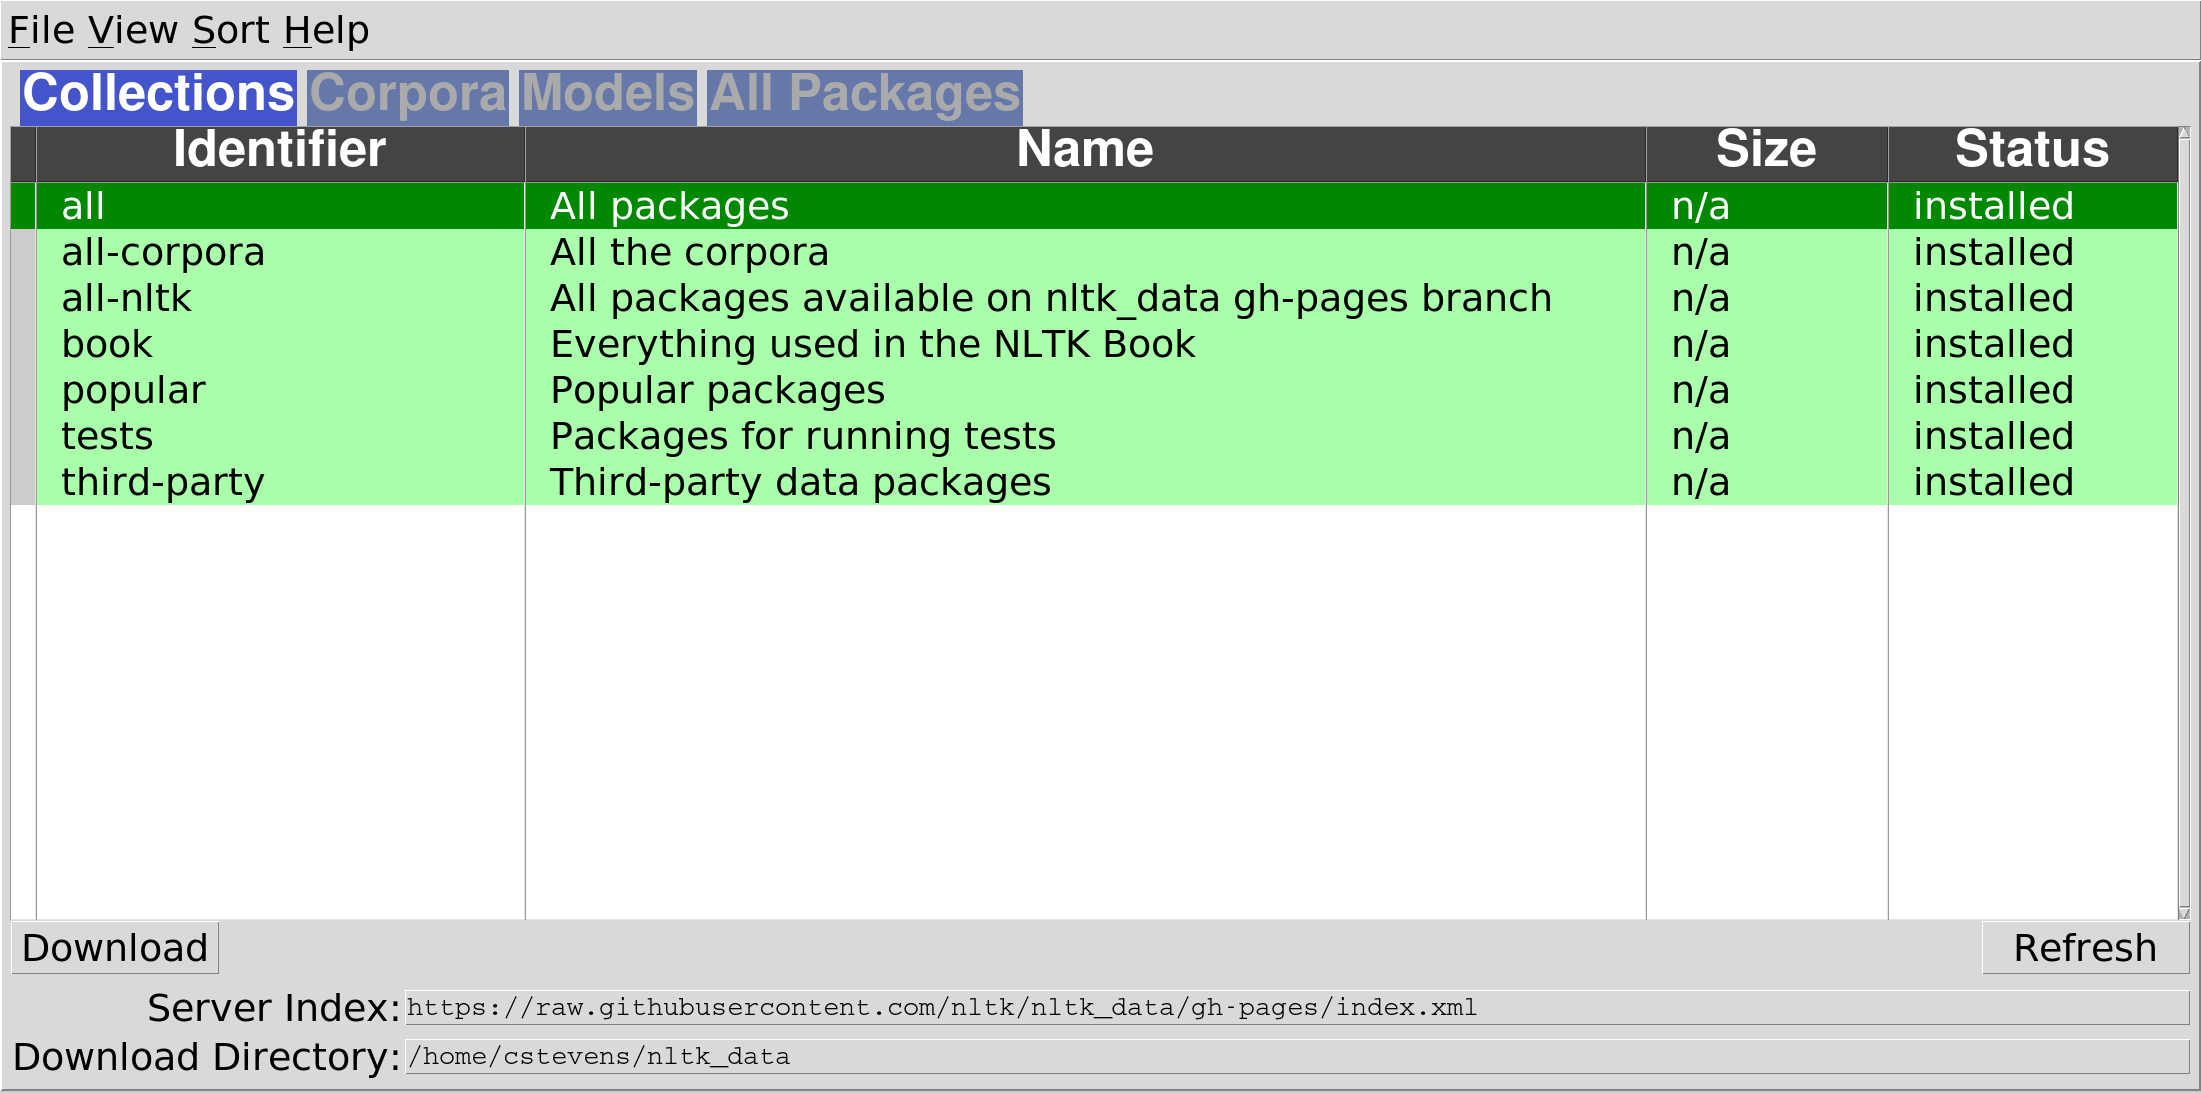
\includegraphics[width=\textwidth]{media/images/nltk_data.png}
  \caption{\textsc{nltk dialog for} installing \textsc{nltk} data packages}
\end{figure*}
\section{running queries}
Once \textsc{python} and \textsc{nltk} are installed you may run queries like
those outlined at the beginning of the article.

First, enter the \textsc{python} environment:
\begin{lstlisting}
  \$ python
\end{lstlisting}
\begin{figure*}[ht]
\centering
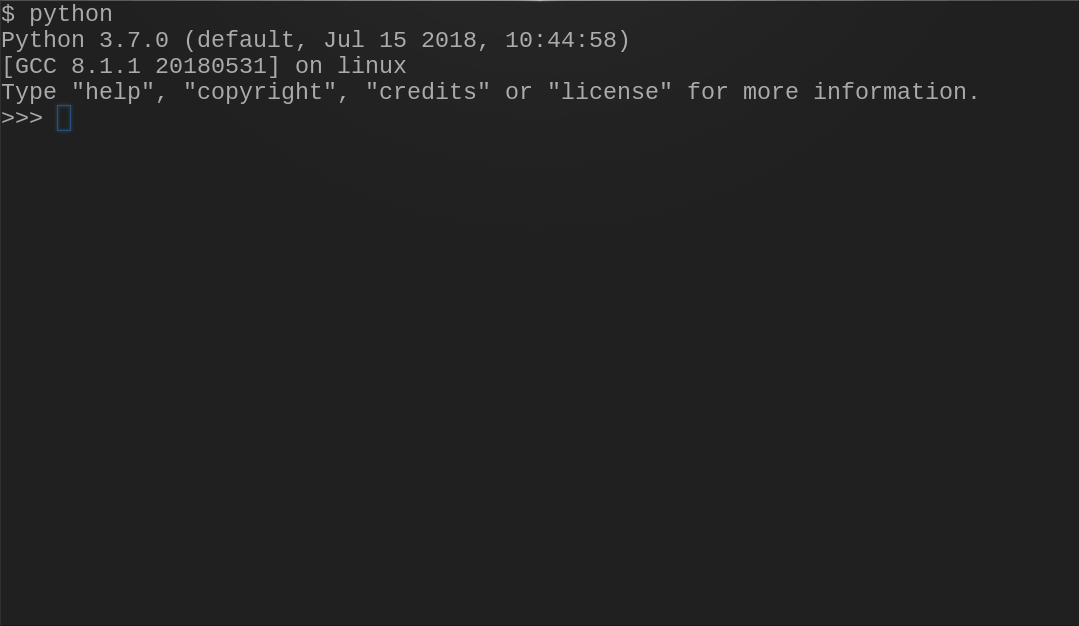
\includegraphics[width=\textwidth]{media/images/python_prompt.png}
  \caption{\textsc{entering the} python environment}
\end{figure*}
Next, we'll load the \textsc{nltk} library and default text corpus included in \textsc{nltk}:
\begin{lstlisting}
  >>> from nltk.book import *
\end{lstlisting}
\begin{figure*}[ht]
\centering
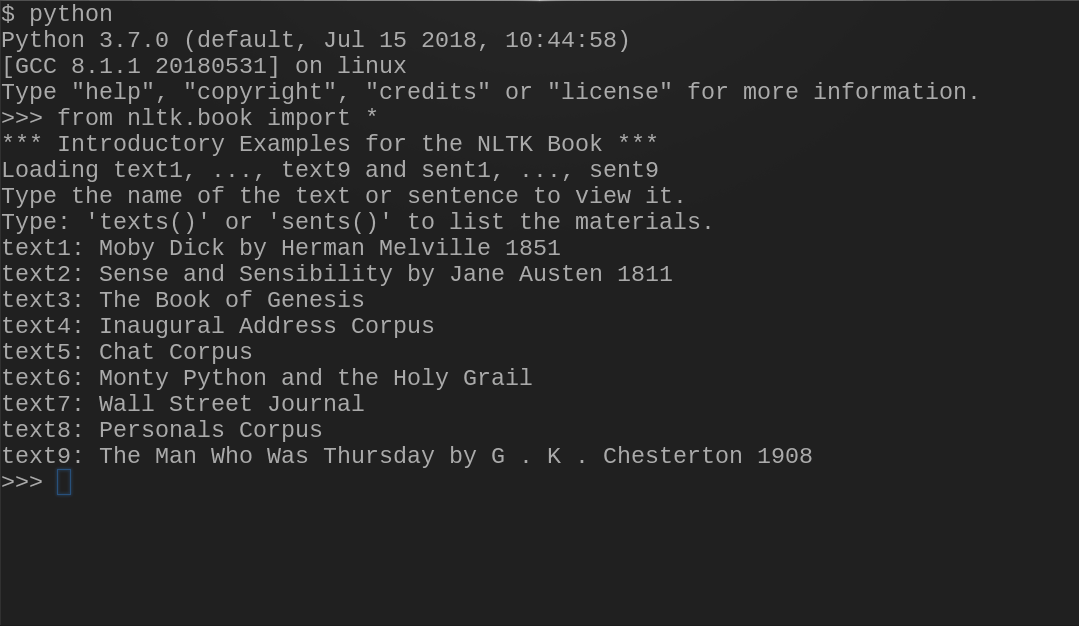
\includegraphics[width=\textwidth]{media/images/nltk_book.png}
  \caption{\textsc{nltk and test data} loaded and ready to receive natural
    language processing requests}
\end{figure*}
Notice the \texttt{\small{text1:, text2:,}} etc. designations. We use these designations
to specify a corpus we'd like to use when querying the data:
\begin{lstlisting}[language=Python]
  >>> text1.concordance('ahab',lines=2)
\end{lstlisting}
\begin{figure*}[ht]
\centering
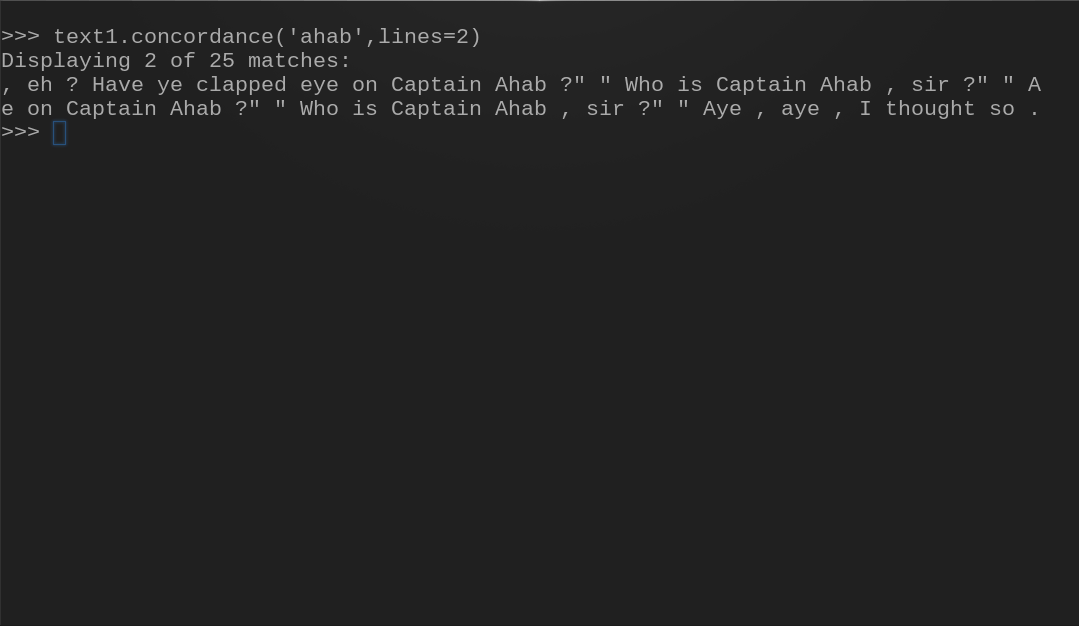
\includegraphics[width=\textwidth]{media/images/python_concord.png}
  \caption{\textsc{querying the 'moby dick'} corpus with the word, 'ahab'}
\end{figure*}
\textsc{nltk} lets you query different types of source data for
different purposes. Perhaps one character in your narrative is a romantic; you
could get insight into his personality by querying a work like
Shakespeare's \textit{Hamlet}. Alternatively, a powerful general may
be best served by \textit{Secret of the Night} by Gaston Leroux. Several works
of the same type may also be combined into a single
corpora for an even broader scope of natural language processing responses.
\section{divide and conquer}
These tools, coupled with custom corpus, make it possible to write scripts to search, tag and template hundreds or thousands of
connections automatically for author review and final implementation.
Automating \textsc{nltk} also works when dividing the work into teams. 

For example, after the creators provide the technical staff with the body of
works they wish to reference in their story a natural language processing based
workflow may look something like this:

\begin{itemize}\setlength\itemsep{0em}
\item Technologists code \& test the automation routines to place \textsc{nltk}
  query results into graphs (e.g. \textsc{graphiz}) 
\item Authors review the graphs containing the results and entity relationships for quality
\item Technologists run automation routines to convert the modified graphs into \textsc{tads3} templates
\item Artists \& authors review the output and modify it
\item Beta testers test, and transcripts are re\textendash entered into the
  natural processing loop as required
\end{itemize}
Of course, all the work, of course, is channeled through a revision system so
everyone receives timely updates.